% "Brainwashing case" figure (fig:2), Beth/Neil chip-implant example.
% Corresponds exactly to papers/2026Fear/models/complete_manipulation.mmd --
% see tikz_roundtrip_examples/README.md for the correspondence mapping.
\begin{figure}[h]
\hspace{1cm}
    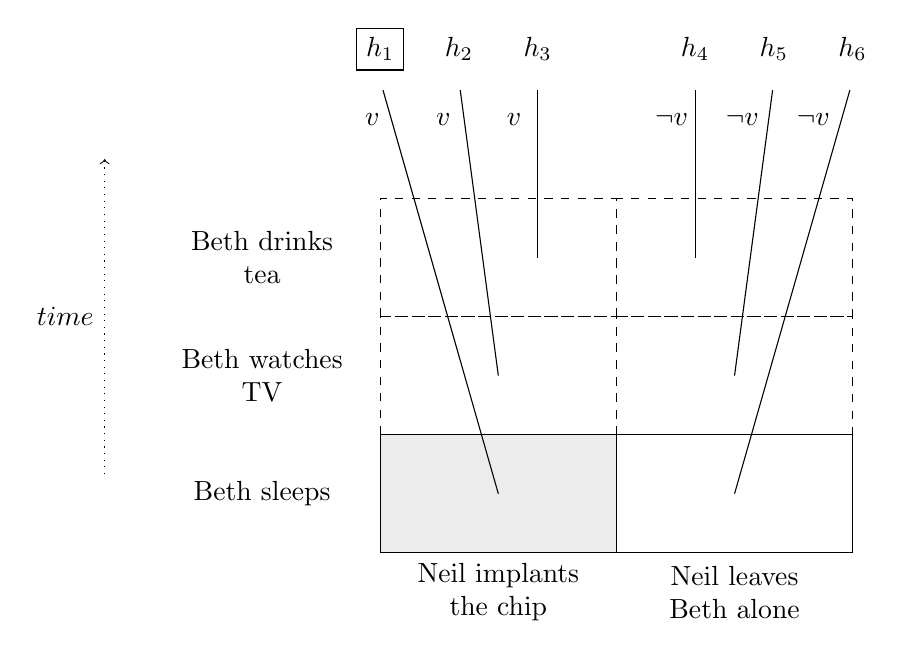
\begin{tikzpicture}
        \draw[->, dotted] (0.5,3) -- (0.5,7); \node at (0,5) {$time$};
        \draw[fill=lightgray!30] (4,2) rectangle (7,3.5); \node[align=center] at (5.5,1.5) {Neil implants\\ the chip};
        \draw (7,2) rectangle (10,3.5); \node[align=center] at (8.5,1.5) {Neil leaves\\ Beth alone};

        \node[align=center] at (2.5,2.75) {Beth sleeps};
        \draw[dashed] (4,3.5) rectangle (7,5); \node[align=center] at (2.5,4.25) {Beth watches\\ TV};
        \draw[dashed] (7,3.5) rectangle (10,5);
        \draw[dashed] (4,5) rectangle (7,6.5); \node[align=center] at (2.5,5.75) {Beth drinks\\ tea};
        \draw[dashed] (7,5) rectangle (10,6.5);

        \node [label={[draw]$h_1$}] (a) at (4, 8) {};
        \node [label={$h_2$}] (b) at (5, 8) {};
        \node [label={$h_3$}] (c) at (6, 8) {};
        \node [label={$h_4$}] (d) at (8, 8) {};
        \node [label={$h_5$}] (e) at (9, 8) {};
        \node [label={$h_6$}] (f) at (10, 8) {};

        \draw (5.5,2.75) -- (a); \node at (3.9,7.5) {$v$};
        \draw (5.5,4.25) -- (b); \node at (4.8,7.5) {$v$};
        \draw (6,5.75) -- (c); \node at (5.7,7.5) {$v$};
        \draw (8,5.75) -- (d); \node at (7.7,7.5) {$\neg v$};
        \draw (8.5,4.25) -- (e); \node at (8.6,7.5) {$\neg v$};
        \draw (8.5,2.75) -- (f); \node at (9.5,7.5) {$\neg v$};
    \end{tikzpicture}
    \caption{Brainwashing case}
    \label{fig:2}
\end{figure}
